Il progetto è stato sviluppato utilizzando \texttt{JavaFX} per la realizzazione dell'interfaccia grafica, adottando una struttura modulare che organizza le classi in package specifici in base al loro ruolo all'interno del progetto. Il funzionamento del progetto, con le relative dipendente, è affidato a \texttt{Maven}.\vspace{.3cm}
Inoltre, per garantire l'affidabilità e il corretto funzionamento delle principali classi del progetto, sono stati implementati test automatizzati utilizzando la libreria \texttt{JUnit} e i relativi metodi \texttt{assert}. Questo approccio ha consentito di identificare e risolvere diversi problemi in fase di implementazioni delle classi.
\subsection{Diagramma dei Package}
\begin{figure}[h]
	\begin{minipage}{0.5\textwidth}
		\centering
		\definecolor{plantucolor0000}{RGB}{0,0,0}
\definecolor{plantucolor0001}{RGB}{241,241,241}
\definecolor{plantucolor0002}{RGB}{24,24,24}
\definecolor{plantucolor0003}{RGB}{173,209,178}
\definecolor{plantucolor0004}{RGB}{180,167,229}

\begin{adjustbox}{width=.5\paperwidth, center}
	\resizebox{\textwidth}{!}{
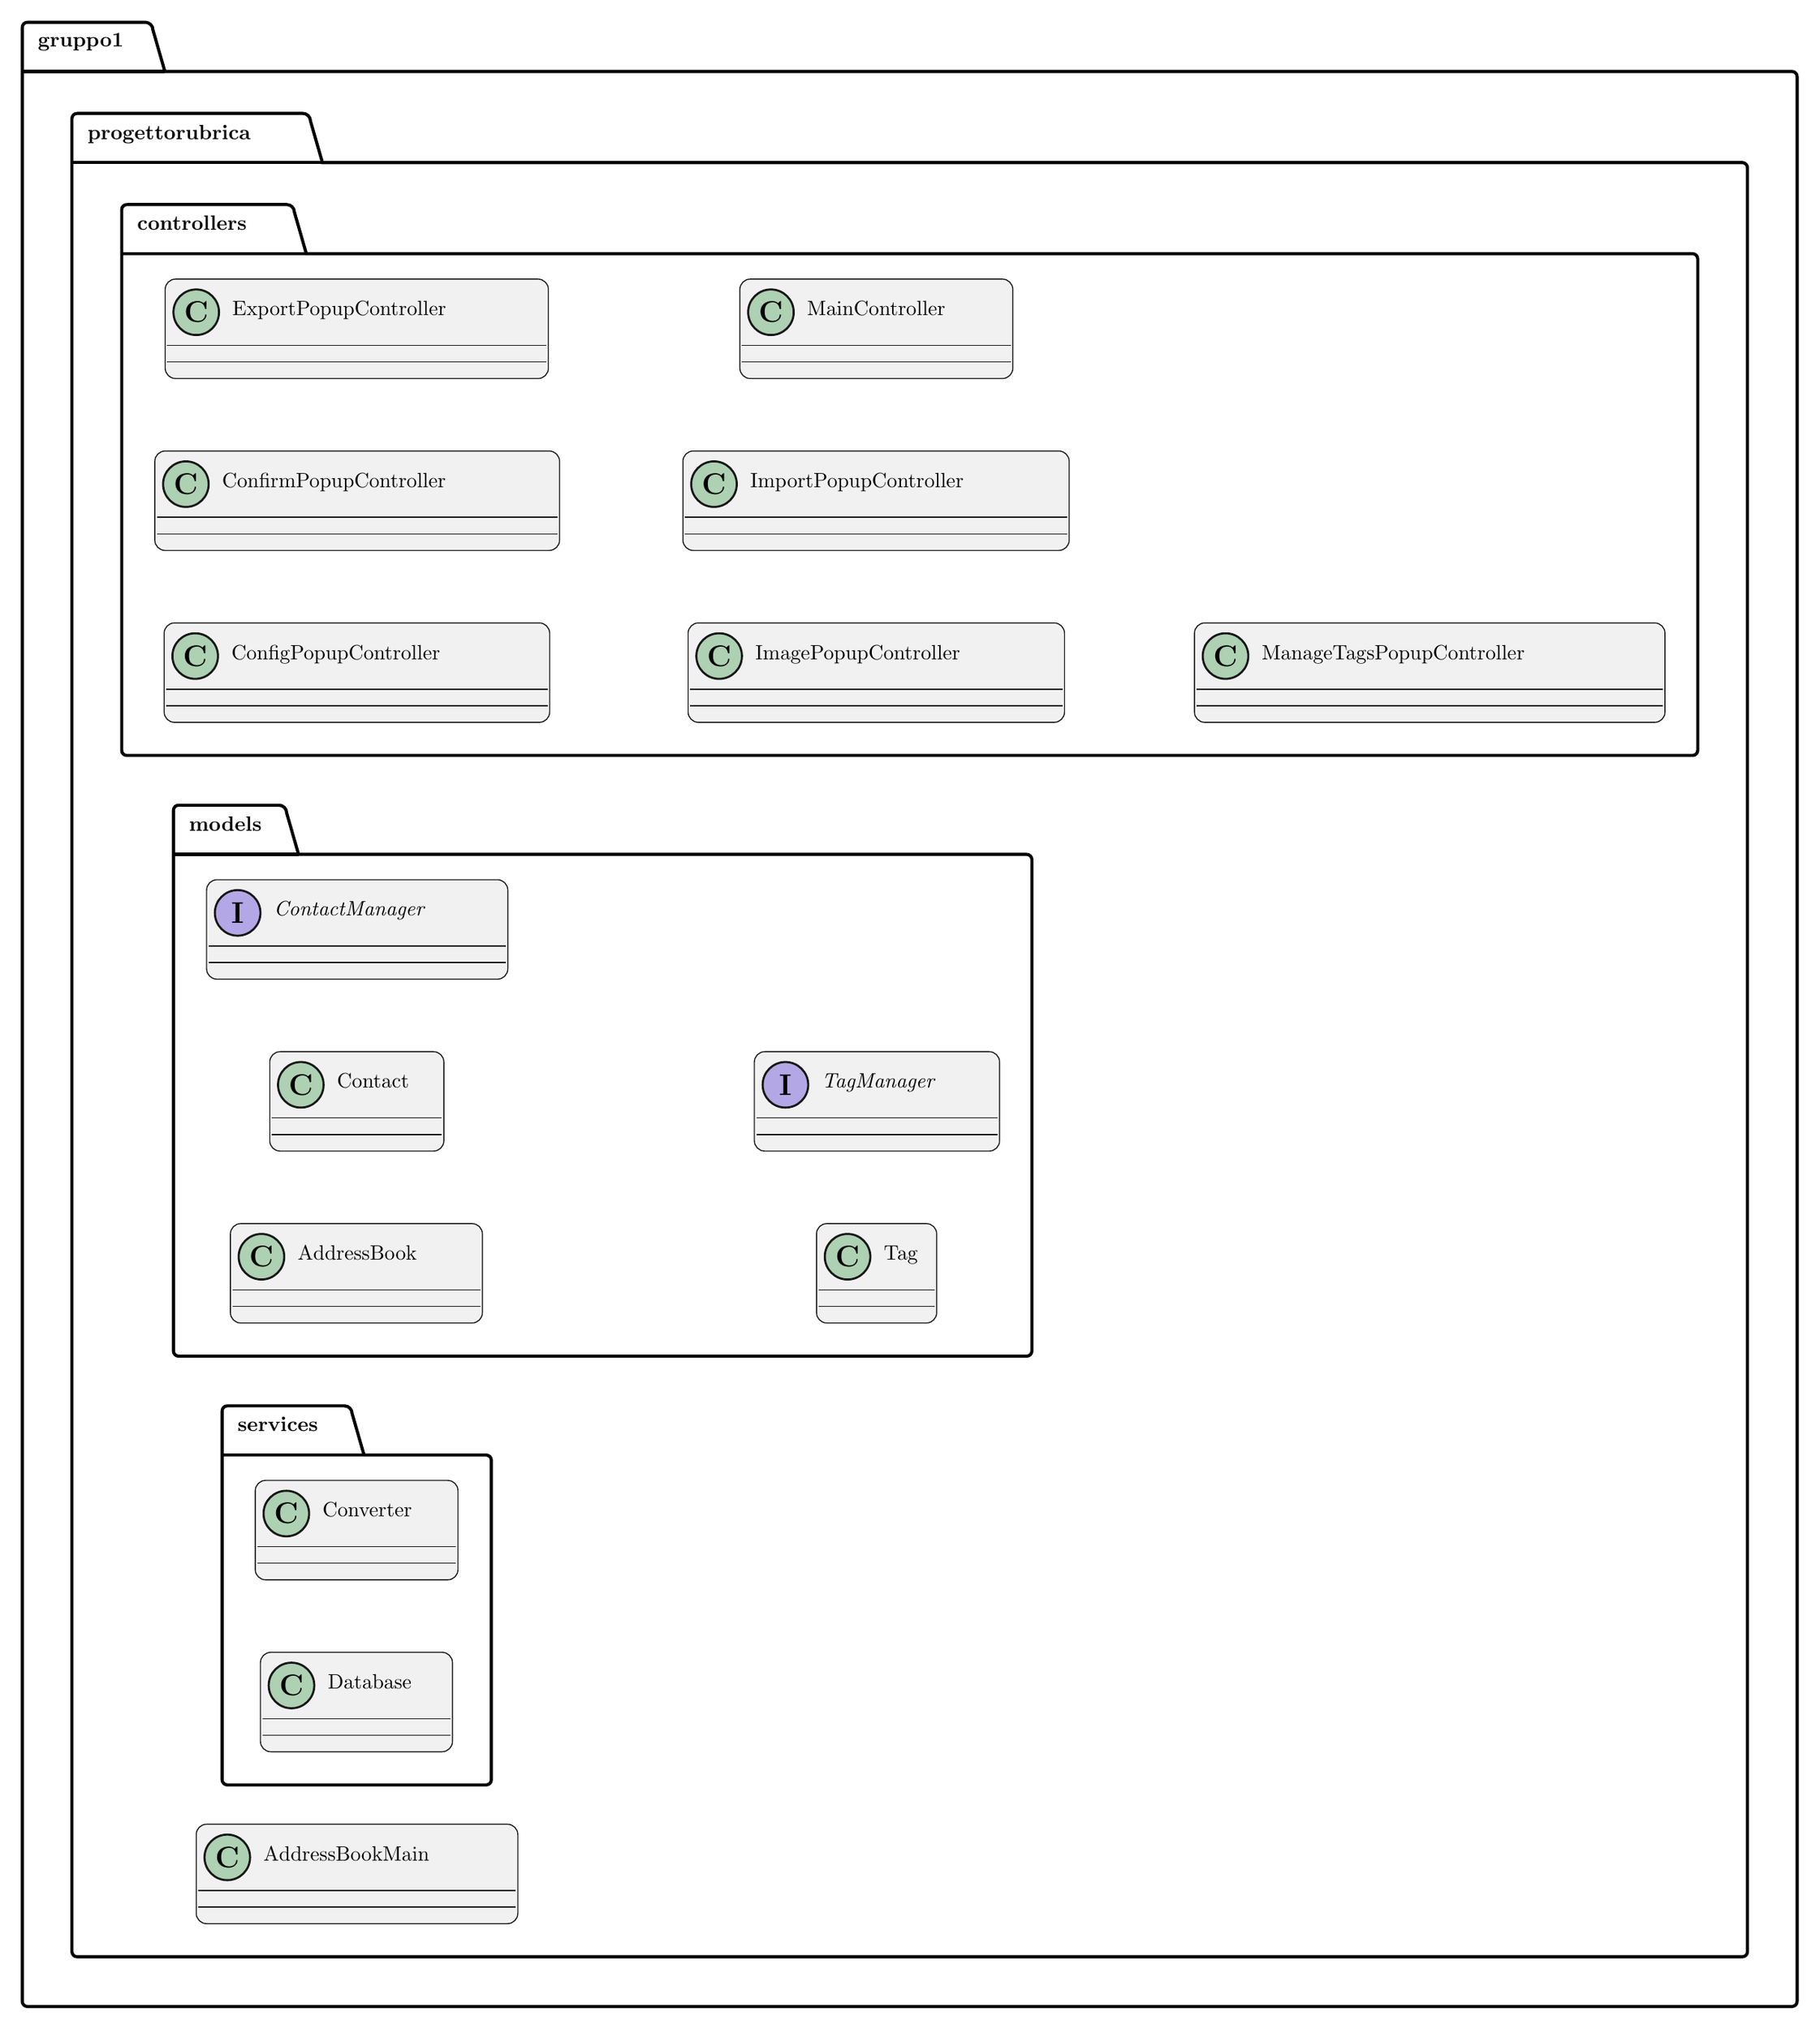
\begin{tikzpicture}[yscale=-1
	,pstyle0/.style={color=black,line width=1.5pt}
	,pstyle1/.style={color=plantucolor0002,fill=plantucolor0001,line width=0.5pt}
	,pstyle2/.style={color=plantucolor0002,fill=plantucolor0003,line width=1.0pt}
	,pstyle3/.style={color=plantucolor0002,line width=0.5pt}
	,pstyle4/.style={color=plantucolor0002,fill=plantucolor0004,line width=1.0pt}
	]
	\draw[pstyle0] (8.5pt,6pt) -- (65.3612pt,6pt) arc(270:360:3.75pt)  -- (74.8612pt,29.7461pt) -- (860.5pt,29.7461pt) arc(270:360:2.5pt)  -- (863pt,961.5pt) arc(0:90:2.5pt)  -- (8.5pt,964pt) arc(90:180:2.5pt)  -- (6pt,8.5pt) arc(180:270:2.5pt) ;
	\draw[pstyle0] (6pt,29.7461pt) -- (74.8612pt,29.7461pt);
	\node at (10pt,8pt)[below right,color=black]{\textbf{gruppo1}};
	\draw[pstyle0] (32.5pt,50pt) -- (141.4368pt,50pt) arc(270:360:3.75pt)  -- (150.9368pt,73.7461pt) -- (836.5pt,73.7461pt) arc(270:360:2.5pt)  -- (839pt,937.5pt) arc(0:90:2.5pt)  -- (32.5pt,940pt) arc(90:180:2.5pt)  -- (30pt,52.5pt) arc(180:270:2.5pt) ;
	\draw[pstyle0] (30pt,73.7461pt) -- (150.9368pt,73.7461pt);
	\node at (34pt,52pt)[below right,color=black]{\textbf{progettorubrica}};
	\draw[pstyle0] (56.5pt,94pt) -- (133.6697pt,94pt) arc(270:360:3.75pt)  -- (143.1697pt,117.7461pt) -- (812.5pt,117.7461pt) arc(270:360:2.5pt)  -- (815pt,357.5pt) arc(0:90:2.5pt)  -- (56.5pt,360pt) arc(90:180:2.5pt)  -- (54pt,96.5pt) arc(180:270:2.5pt) ;
	\draw[pstyle0] (54pt,117.7461pt) -- (143.1697pt,117.7461pt);
	\node at (58pt,96pt)[below right,color=black]{\textbf{controllers}};
	\draw[pstyle0] (81.5pt,384pt) -- (129.914pt,384pt) arc(270:360:3.75pt)  -- (139.414pt,407.7461pt) -- (491pt,407.7461pt) arc(270:360:2.5pt)  -- (493.5pt,647.5pt) arc(0:90:2.5pt)  -- (81.5pt,650pt) arc(90:180:2.5pt)  -- (79pt,386.5pt) arc(180:270:2.5pt) ;
	\draw[pstyle0] (79pt,407.7461pt) -- (139.414pt,407.7461pt);
	\node at (83pt,386pt)[below right,color=black]{\textbf{models}};
	\draw[pstyle0] (105pt,674pt) -- (161.5347pt,674pt) arc(270:360:3.75pt)  -- (171.0347pt,697.7461pt) -- (230pt,697.7461pt) arc(270:360:2.5pt)  -- (232.5pt,854.5pt) arc(0:90:2.5pt)  -- (105pt,857pt) arc(90:180:2.5pt)  -- (102.5pt,676.5pt) arc(180:270:2.5pt) ;
	\draw[pstyle0] (102.5pt,697.7461pt) -- (171.0347pt,697.7461pt);
	\node at (106.5pt,676pt)[below right,color=black]{\textbf{services}};
	\draw[pstyle1] (90pt,881pt) arc (180:270:5pt) -- (95pt,876pt) -- (240.2893pt,876pt) arc (270:360:5pt) -- (245.2893pt,881pt) -- (245.2893pt,919pt) arc (0:90:5pt) -- (240.2893pt,924pt) -- (95pt,924pt) arc (90:180:5pt) -- (90pt,919pt) -- cycle;
	\draw[pstyle2] (105pt,892pt) ellipse (11pt and 11pt);
	\node at (105pt,892pt)[]{\textbf{\Large C}};
	\node at (119pt,883.127pt)[below right,color=black]{AddressBookMain};
	\draw[pstyle3] (91pt,908pt) -- (244.2893pt,908pt);
	\draw[pstyle3] (91pt,916pt) -- (244.2893pt,916pt);
	\draw[pstyle1] (74.5pt,301pt) arc (180:270:5pt) -- (79.5pt,296pt) -- (255.6538pt,296pt) arc (270:360:5pt) -- (260.6538pt,301pt) -- (260.6538pt,339pt) arc (0:90:5pt) -- (255.6538pt,344pt) -- (79.5pt,344pt) arc (90:180:5pt) -- (74.5pt,339pt) -- cycle;
	\draw[pstyle2] (89.5pt,312pt) ellipse (11pt and 11pt);
	\node at (89.5pt,312pt)[]{\textbf{\Large C}};
	\node at (103.5pt,303.127pt)[below right,color=black]{ConfigPopupController};
	\draw[pstyle3] (75.5pt,328pt) -- (259.6538pt,328pt);
	\draw[pstyle3] (75.5pt,336pt) -- (259.6538pt,336pt);
	\draw[pstyle1] (70pt,218pt) arc (180:270:5pt) -- (75pt,213pt) -- (260.4331pt,213pt) arc (270:360:5pt) -- (265.4331pt,218pt) -- (265.4331pt,256pt) arc (0:90:5pt) -- (260.4331pt,261pt) -- (75pt,261pt) arc (90:180:5pt) -- (70pt,256pt) -- cycle;
	\draw[pstyle2] (85pt,229pt) ellipse (11pt and 11pt);
	\node at (85pt,229pt)[]{\textbf{\Large C}};
	\node at (99pt,220.127pt)[below right,color=black]{ConfirmPopupController};
	\draw[pstyle3] (71pt,245pt) -- (264.4331pt,245pt);
	\draw[pstyle3] (71pt,253pt) -- (264.4331pt,253pt);
	\draw[pstyle1] (75pt,135pt) arc (180:270:5pt) -- (80pt,130pt) -- (255.0462pt,130pt) arc (270:360:5pt) -- (260.0462pt,135pt) -- (260.0462pt,173pt) arc (0:90:5pt) -- (255.0462pt,178pt) -- (80pt,178pt) arc (90:180:5pt) -- (75pt,173pt) -- cycle;
	\draw[pstyle2] (90pt,146pt) ellipse (11pt and 11pt);
	\node at (90pt,146pt)[]{\textbf{\Large C}};
	\node at (104pt,137.127pt)[below right,color=black]{ExportPopupController};
	\draw[pstyle3] (76pt,162pt) -- (259.0462pt,162pt);
	\draw[pstyle3] (76pt,170pt) -- (259.0462pt,170pt);
	\draw[pstyle1] (327.5pt,301pt) arc (180:270:5pt) -- (332.5pt,296pt) -- (504.2543pt,296pt) arc (270:360:5pt) -- (509.2543pt,301pt) -- (509.2543pt,339pt) arc (0:90:5pt) -- (504.2543pt,344pt) -- (332.5pt,344pt) arc (90:180:5pt) -- (327.5pt,339pt) -- cycle;
	\draw[pstyle2] (342.5pt,312pt) ellipse (11pt and 11pt);
	\node at (342.5pt,312pt)[]{\textbf{\Large C}};
	\node at (356.5pt,303.127pt)[below right,color=black]{ImagePopupController};
	\draw[pstyle3] (328.5pt,328pt) -- (508.2543pt,328pt);
	\draw[pstyle3] (328.5pt,336pt) -- (508.2543pt,336pt);
	\draw[pstyle1] (325pt,218pt) arc (180:270:5pt) -- (330pt,213pt) -- (506.513pt,213pt) arc (270:360:5pt) -- (511.513pt,218pt) -- (511.513pt,256pt) arc (0:90:5pt) -- (506.513pt,261pt) -- (330pt,261pt) arc (90:180:5pt) -- (325pt,256pt) -- cycle;
	\draw[pstyle2] (340pt,229pt) ellipse (11pt and 11pt);
	\node at (340pt,229pt)[]{\textbf{\Large C}};
	\node at (354pt,220.127pt)[below right,color=black]{ImportPopupController};
	\draw[pstyle3] (326pt,245pt) -- (510.513pt,245pt);
	\draw[pstyle3] (326pt,253pt) -- (510.513pt,253pt);
	\draw[pstyle1] (352.5pt,135pt) arc (180:270:5pt) -- (357.5pt,130pt) -- (479.3pt,130pt) arc (270:360:5pt) -- (484.3pt,135pt) -- (484.3pt,173pt) arc (0:90:5pt) -- (479.3pt,178pt) -- (357.5pt,178pt) arc (90:180:5pt) -- (352.5pt,173pt) -- cycle;
	\draw[pstyle2] (367.5pt,146pt) ellipse (11pt and 11pt);
	\node at (367.5pt,146pt)[]{\textbf{\Large C}};
	\node at (381.5pt,137.127pt)[below right,color=black]{MainController};
	\draw[pstyle3] (353.5pt,162pt) -- (483.3pt,162pt);
	\draw[pstyle3] (353.5pt,170pt) -- (483.3pt,170pt);
	\draw[pstyle1] (572pt,301pt) arc (180:270:5pt) -- (577pt,296pt) -- (794.2146pt,296pt) arc (270:360:5pt) -- (799.2146pt,301pt) -- (799.2146pt,339pt) arc (0:90:5pt) -- (794.2146pt,344pt) -- (577pt,344pt) arc (90:180:5pt) -- (572pt,339pt) -- cycle;
	\draw[pstyle2] (587pt,312pt) ellipse (11pt and 11pt);
	\node at (587pt,312pt)[]{\textbf{\Large C}};
	\node at (601pt,303.127pt)[below right,color=black]{ManageTagsPopupController};
	\draw[pstyle3] (573pt,328pt) -- (798.2146pt,328pt);
	\draw[pstyle3] (573pt,336pt) -- (798.2146pt,336pt);
	\draw[pstyle1] (106.5pt,591pt) arc (180:270:5pt) -- (111.5pt,586pt) -- (223.18pt,586pt) arc (270:360:5pt) -- (228.18pt,591pt) -- (228.18pt,629pt) arc (0:90:5pt) -- (223.18pt,634pt) -- (111.5pt,634pt) arc (90:180:5pt) -- (106.5pt,629pt) -- cycle;
	\draw[pstyle2] (121.5pt,602pt) ellipse (11pt and 11pt);
	\node at (121.5pt,602pt)[]{\textbf{\Large C}};
	\node at (135.5pt,593.127pt)[below right,color=black]{AddressBook};
	\draw[pstyle3] (107.5pt,618pt) -- (227.18pt,618pt);
	\draw[pstyle3] (107.5pt,626pt) -- (227.18pt,626pt);
	\draw[pstyle1] (125.5pt,508pt) arc (180:270:5pt) -- (130.5pt,503pt) -- (204.5727pt,503pt) arc (270:360:5pt) -- (209.5727pt,508pt) -- (209.5727pt,546pt) arc (0:90:5pt) -- (204.5727pt,551pt) -- (130.5pt,551pt) arc (90:180:5pt) -- (125.5pt,546pt) -- cycle;
	\draw[pstyle2] (140.5pt,519pt) ellipse (11pt and 11pt);
	\node at (140.5pt,519pt)[]{\textbf{\Large C}};
	\node at (154.5pt,510.127pt)[below right,color=black]{Contact};
	\draw[pstyle3] (126.5pt,535pt) -- (208.5727pt,535pt);
	\draw[pstyle3] (126.5pt,543pt) -- (208.5727pt,543pt);
	\draw[pstyle1] (95pt,425pt) arc (180:270:5pt) -- (100pt,420pt) -- (235.4526pt,420pt) arc (270:360:5pt) -- (240.4526pt,425pt) -- (240.4526pt,463pt) arc (0:90:5pt) -- (235.4526pt,468pt) -- (100pt,468pt) arc (90:180:5pt) -- (95pt,463pt) -- cycle;
	\draw[pstyle4] (110pt,436pt) ellipse (11pt and 11pt);
	\node at (110pt,436pt)[]{\textbf{\Large I}};
	\node at (124pt,427.127pt)[below right,color=black]{\textit{ContactManager}};
	\draw[pstyle3] (96pt,452pt) -- (239.4526pt,452pt);
	\draw[pstyle3] (96pt,460pt) -- (239.4526pt,460pt);
	\draw[pstyle1] (389.5pt,591pt) arc (180:270:5pt) -- (394.5pt,586pt) -- (442.5364pt,586pt) arc (270:360:5pt) -- (447.5364pt,591pt) -- (447.5364pt,629pt) arc (0:90:5pt) -- (442.5364pt,634pt) -- (394.5pt,634pt) arc (90:180:5pt) -- (389.5pt,629pt) -- cycle;
	\draw[pstyle2] (404.5pt,602pt) ellipse (11pt and 11pt);
	\node at (404.5pt,602pt)[]{\textbf{\Large C}};
	\node at (418.5pt,593.127pt)[below right,color=black]{Tag};
	\draw[pstyle3] (390.5pt,618pt) -- (446.5364pt,618pt);
	\draw[pstyle3] (390.5pt,626pt) -- (446.5364pt,626pt);
	\draw[pstyle1] (359.5pt,508pt) arc (180:270:5pt) -- (364.5pt,503pt) -- (472.8945pt,503pt) arc (270:360:5pt) -- (477.8945pt,508pt) -- (477.8945pt,546pt) arc (0:90:5pt) -- (472.8945pt,551pt) -- (364.5pt,551pt) arc (90:180:5pt) -- (359.5pt,546pt) -- cycle;
	\draw[pstyle4] (374.5pt,519pt) ellipse (11pt and 11pt);
	\node at (374.5pt,519pt)[]{\textbf{\Large I}};
	\node at (388.5pt,510.127pt)[below right,color=black]{\textit{TagManager}};
	\draw[pstyle3] (360.5pt,535pt) -- (476.8945pt,535pt);
	\draw[pstyle3] (360.5pt,543pt) -- (476.8945pt,543pt);
	\draw[pstyle1] (118.5pt,715pt) arc (180:270:5pt) -- (123.5pt,710pt) -- (211.4143pt,710pt) arc (270:360:5pt) -- (216.4143pt,715pt) -- (216.4143pt,753pt) arc (0:90:5pt) -- (211.4143pt,758pt) -- (123.5pt,758pt) arc (90:180:5pt) -- (118.5pt,753pt) -- cycle;
	\draw[pstyle2] (133.5pt,726pt) ellipse (11pt and 11pt);
	\node at (133.5pt,726pt)[]{\textbf{\Large C}};
	\node at (147.5pt,717.127pt)[below right,color=black]{Converter};
	\draw[pstyle3] (119.5pt,742pt) -- (215.4143pt,742pt);
	\draw[pstyle3] (119.5pt,750pt) -- (215.4143pt,750pt);
	\draw[pstyle1] (121pt,798pt) arc (180:270:5pt) -- (126pt,793pt) -- (208.7294pt,793pt) arc (270:360:5pt) -- (213.7294pt,798pt) -- (213.7294pt,836pt) arc (0:90:5pt) -- (208.7294pt,841pt) -- (126pt,841pt) arc (90:180:5pt) -- (121pt,836pt) -- cycle;
	\draw[pstyle2] (136pt,809pt) ellipse (11pt and 11pt);
	\node at (136pt,809pt)[]{\textbf{\Large C}};
	\node at (150pt,800.127pt)[below right,color=black]{Database};
	\draw[pstyle3] (122pt,825pt) -- (212.7294pt,825pt);
	\draw[pstyle3] (122pt,833pt) -- (212.7294pt,833pt);
\end{tikzpicture}
}
\end{adjustbox}
		\caption{Diagramma package implementazione}
		\label{fig:diagramma-package-implementazione}
	\end{minipage}%
	\hfill
	\begin{minipage}{0.5\textwidth}
		\centering
		\definecolor{plantucolor0000}{RGB}{0,0,0}
\definecolor{plantucolor0001}{RGB}{241,241,241}
\definecolor{plantucolor0002}{RGB}{24,24,24}
\definecolor{plantucolor0003}{RGB}{173,209,178}

\begin{adjustbox}{width=.3\paperwidth, center}
	\resizebox{\textwidth}{!}{
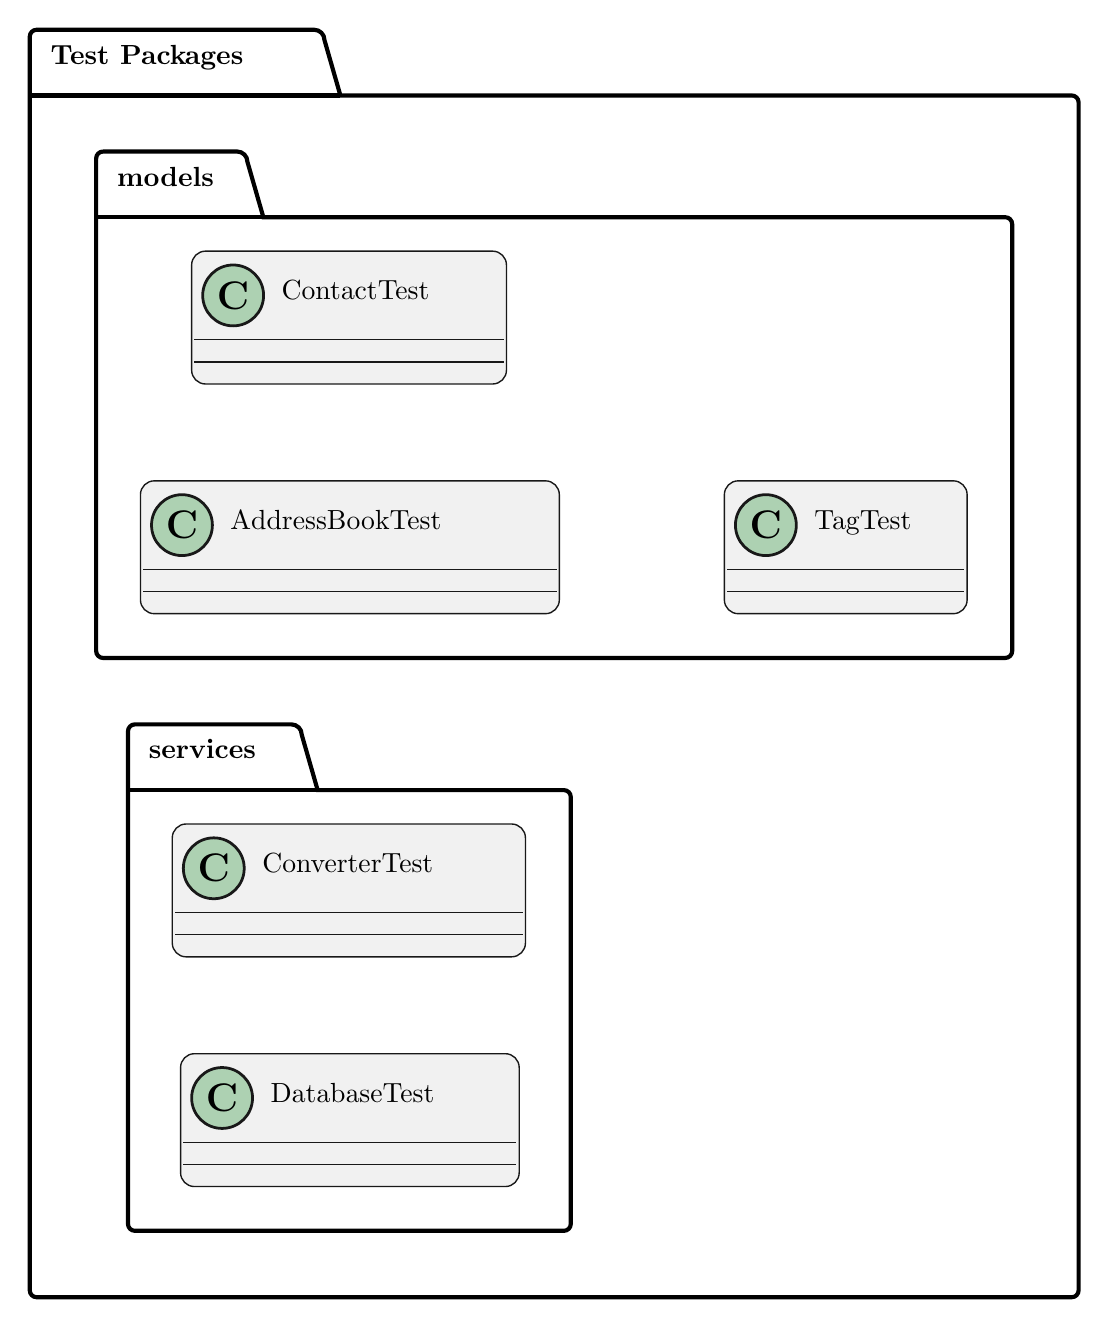
\begin{tikzpicture}[yscale=-1
,pstyle0/.style={color=black,line width=1.5pt}
,pstyle1/.style={color=plantucolor0002,fill=plantucolor0001,line width=0.5pt}
,pstyle2/.style={color=plantucolor0002,fill=plantucolor0003,line width=1.0pt}
,pstyle3/.style={color=plantucolor0002,line width=0.5pt}
]
\draw[pstyle0] (8.5pt,6pt) -- (108.7506pt,6pt) arc(270:360:3.75pt)  -- (118.2506pt,29.7461pt) -- (382.5pt,29.7461pt) arc(270:360:2.5pt)  -- (385pt,461.5pt) arc(0:90:2.5pt)  -- (8.5pt,464pt) arc(90:180:2.5pt)  -- (6pt,8.5pt) arc(180:270:2.5pt) ;
\draw[pstyle0] (6pt,29.7461pt) -- (118.2506pt,29.7461pt);
\node at (10pt,8pt)[below right,color=black]{\textbf{Test Packages}};
\draw[pstyle0] (32.5pt,50pt) -- (80.914pt,50pt) arc(270:360:3.75pt)  -- (90.414pt,73.7461pt) -- (358.5pt,73.7461pt) arc(270:360:2.5pt)  -- (361pt,230.5pt) arc(0:90:2.5pt)  -- (32.5pt,233pt) arc(90:180:2.5pt)  -- (30pt,52.5pt) arc(180:270:2.5pt) ;
\draw[pstyle0] (30pt,73.7461pt) -- (90.414pt,73.7461pt);
\node at (34pt,52pt)[below right,color=black]{\textbf{models}};
\draw[pstyle0] (44pt,257pt) -- (100.5347pt,257pt) arc(270:360:3.75pt)  -- (110.0347pt,280.7461pt) -- (199pt,280.7461pt) arc(270:360:2.5pt)  -- (201.5pt,437.5pt) arc(0:90:2.5pt)  -- (44pt,440pt) arc(90:180:2.5pt)  -- (41.5pt,259.5pt) arc(180:270:2.5pt) ;
\draw[pstyle0] (41.5pt,280.7461pt) -- (110.0347pt,280.7461pt);
\node at (45.5pt,259pt)[below right,color=black]{\textbf{services}};
\draw[pstyle1] (46pt,174pt) arc (180:270:5pt) -- (51pt,169pt) -- (192.36pt,169pt) arc (270:360:5pt) -- (197.36pt,174pt) -- (197.36pt,212pt) arc (0:90:5pt) -- (192.36pt,217pt) -- (51pt,217pt) arc (90:180:5pt) -- (46pt,212pt) -- cycle;
\draw[pstyle2] (61pt,185pt) ellipse (11pt and 11pt);
\node at (61pt,185pt)[]{\textbf{\Large C}};
\node at (75pt,176.127pt)[below right,color=black]{AddressBookTest};
\draw[pstyle3] (47pt,201pt) -- (196.36pt,201pt);
\draw[pstyle3] (47pt,209pt) -- (196.36pt,209pt);
\draw[pstyle1] (64.5pt,91pt) arc (180:270:5pt) -- (69.5pt,86pt) -- (173.2565pt,86pt) arc (270:360:5pt) -- (178.2565pt,91pt) -- (178.2565pt,129pt) arc (0:90:5pt) -- (173.2565pt,134pt) -- (69.5pt,134pt) arc (90:180:5pt) -- (64.5pt,129pt) -- cycle;
\draw[pstyle2] (79.5pt,102pt) ellipse (11pt and 11pt);
\node at (79.5pt,102pt)[]{\textbf{\Large C}};
\node at (93.5pt,93.127pt)[below right,color=black]{ContactTest};
\draw[pstyle3] (65.5pt,118pt) -- (177.2565pt,118pt);
\draw[pstyle3] (65.5pt,126pt) -- (177.2565pt,126pt);
\draw[pstyle1] (257pt,174pt) arc (180:270:5pt) -- (262pt,169pt) -- (339.7191pt,169pt) arc (270:360:5pt) -- (344.7191pt,174pt) -- (344.7191pt,212pt) arc (0:90:5pt) -- (339.7191pt,217pt) -- (262pt,217pt) arc (90:180:5pt) -- (257pt,212pt) -- cycle;
\draw[pstyle2] (272pt,185pt) ellipse (11pt and 11pt);
\node at (272pt,185pt)[]{\textbf{\Large C}};
\node at (286pt,176.127pt)[below right,color=black]{TagTest};
\draw[pstyle3] (258pt,201pt) -- (343.7191pt,201pt);
\draw[pstyle3] (258pt,209pt) -- (343.7191pt,209pt);
\draw[pstyle1] (57.5pt,298pt) arc (180:270:5pt) -- (62.5pt,293pt) -- (180.1198pt,293pt) arc (270:360:5pt) -- (185.1198pt,298pt) -- (185.1198pt,336pt) arc (0:90:5pt) -- (180.1198pt,341pt) -- (62.5pt,341pt) arc (90:180:5pt) -- (57.5pt,336pt) -- cycle;
\draw[pstyle2] (72.5pt,309pt) ellipse (11pt and 11pt);
\node at (72.5pt,309pt)[]{\textbf{\Large C}};
\node at (86.5pt,300.127pt)[below right,color=black]{ConverterTest};
\draw[pstyle3] (58.5pt,325pt) -- (184.1198pt,325pt);
\draw[pstyle3] (58.5pt,333pt) -- (184.1198pt,333pt);
\draw[pstyle1] (60.5pt,381pt) arc (180:270:5pt) -- (65.5pt,376pt) -- (177.8579pt,376pt) arc (270:360:5pt) -- (182.8579pt,381pt) -- (182.8579pt,419pt) arc (0:90:5pt) -- (177.8579pt,424pt) -- (65.5pt,424pt) arc (90:180:5pt) -- (60.5pt,419pt) -- cycle;
\draw[pstyle2] (75.5pt,392pt) ellipse (11pt and 11pt);
\node at (75.5pt,392pt)[]{\textbf{\Large C}};
\node at (89.5pt,383.127pt)[below right,color=black]{DatabaseTest};
\draw[pstyle3] (61.5pt,408pt) -- (181.8579pt,408pt);
\draw[pstyle3] (61.5pt,416pt) -- (181.8579pt,416pt);
\end{tikzpicture}
}
\end{adjustbox}
		\caption{Diagramma package testing}
		\label{fig:diagramma-package-testing}
	\end{minipage}
\end{figure}

\begin{tcolorbox}[colback=white,colframe=black!80!white,title=\textbf{Package controllers}]
	Questo Package è dedicato esclusivamente alla gestione dell'interfaccia grafica dell'applicazione. Al suo interno sono presenti classi Controller ognuna delle quali gestisce un aspetto specifico dell'interfaccia grafica, come l'esportazione (\textit{ExportPopupController}), importazione (\textit{ImportPopupController}) o schermata di conferma per l'eliminazione di un contatto o tag (\textit{ConfirmPopupController}). \\
	Questo consente una separazione delle responsabilità, con i controller che si occupano esclusivamente della logica di interazione con l'utente.
	\\La presenza di diverse classi, ciascuna con un compito preciso, segue il principio di singola responsabilità.
\end{tcolorbox}

\begin{tcolorbox}[colback=white,colframe=black!80!white,title=\textbf{Package models}]
	Questo Package contiene le classi che rappresentano i modelli del sistema e la logica. 
	\\Definendo \textit{AddressBook}, \textit{Contact} e \textit{Tag} si definiscono i modelli.
	\\Definendo le interfacce \textit{ContactManager} e \textit{TagManager} si separa la gestione dei modelli e le interazioni con questi. \\
	Tali interfacce offrono dei metodi per \textit{ExportPopupController}, \textit{ImportPopupController} e \textit{ManageTagsPopupController} per la gestione dei contatti e dei tag.
\end{tcolorbox}

\begin{tcolorbox}[colback=white,colframe=black!80!white,title=\textbf{Package services}]
	In questo Package sono presenti le classi \textit{Converter} e \textit{Database}, che gestiscono operazioni generali come la conversione di dati e l'interazione con il database. \\
	Tali classi si occupano del salvataggio dei dati in remoto e la trasformazione dei formati.
	Questo riduce la duplicazione del codice e quindi migliora la manutenibilità.
\end{tcolorbox}

\begin{tcolorbox}[colback=white,colframe=black!80!white,title=\textbf{Package di test}]
	I Package per i test sono relativi ai modelli e ai servizi e sono in un package separato. \\
	Le classi di test AddressBookTest, ContactTest e TagTest sono associati ai rispettivi modelli, mentre ConverterTest e DatabaseTest sono dedicati ai test dei servizi.\\
	Questo facilita l'individuazione di eventuali bug in fase di implementazione e refactoring.
\end{tcolorbox}

\newpage
\subsection{UTC 1 - AddressBook}
\begin{center} \includegraphics[width=\linewidth]{images/UTC/1-1.png} \end{center}
\begin{center} \includegraphics[width=\linewidth]{images/UTC/1-2.png} \end{center}
\begin{center} \includegraphics[width=\linewidth]{images/UTC/1-8.png} \end{center}
\begin{center} \includegraphics[width=\linewidth]{images/UTC/1-4.png} \end{center}
\begin{center} \includegraphics[width=\linewidth]{images/UTC/1-9.png} \end{center}
\begin{center} \includegraphics[width=\linewidth]{images/UTC/1-10.png} \end{center}
\begin{center} \includegraphics[width=\linewidth]{images/UTC/1-12.png} \end{center}
\begin{center} \includegraphics[width=\linewidth]{images/UTC/1-14.png} \end{center}
\begin{center} \includegraphics[width=\linewidth]{images/UTC/1-15.png} \end{center}
\subsection{UTC 2 - Contact}
\begin{center} \includegraphics[width=\linewidth]{images/UTC/2-16.png} \end{center}
\begin{center} \includegraphics[width=\linewidth]{images/UTC/2-17.png} \end{center}
\begin{center} \includegraphics[width=\linewidth]{images/UTC/2-18.png} \end{center}
\subsection{UTC 3 - Converter}
\begin{center} \includegraphics[width=\linewidth]{images/UTC/3-1.png} \end{center}
\begin{center} \includegraphics[width=\linewidth]{images/UTC/3-2.png} \end{center}
\begin{center} \includegraphics[width=\linewidth]{images/UTC/3-4.png} \end{center}
\begin{center} \includegraphics[width=\linewidth]{images/UTC/3-5.png} \end{center}
\begin{center} \includegraphics[width=\linewidth]{images/UTC/3-6.png} \end{center}
\begin{center} \includegraphics[width=\linewidth]{images/UTC/3-8.png} \end{center}
\begin{center} \includegraphics[width=\linewidth]{images/UTC/3-9.png} \end{center}
\begin{center} \includegraphics[width=\linewidth]{images/UTC/3-10.png} \end{center}
\begin{center} \includegraphics[width=\linewidth]{images/UTC/3-11.png} \end{center}
\begin{center} \includegraphics[width=\linewidth]{images/UTC/3-12.png} \end{center}
\begin{center} \includegraphics[width=\linewidth]{images/UTC/3-13.png} \end{center}
\begin{center} \includegraphics[width=\linewidth]{images/UTC/3.14.png} \end{center}
\begin{center} \includegraphics[width=\linewidth]{images/UTC/3.16.png} \end{center}
\begin{center} \includegraphics[width=\linewidth]{images/UTC/3.18.png} \end{center}
\begin{center} \includegraphics[width=\linewidth]{images/UTC/3.19.png} \end{center}
\subsection{UTC 4 - Database}
\begin{center} \includegraphics[width=\linewidth]{images/UTC/4.2.png} \end{center}
\begin{center} \includegraphics[width=\linewidth]{images/UTC/4.3.png} \end{center}
\begin{center} \includegraphics[width=\linewidth]{images/UTC/4.4.png} \end{center}
\begin{center} \includegraphics[width=\linewidth]{images/UTC/4.5.png} \end{center}
\begin{center} \includegraphics[width=\linewidth]{images/UTC/4.6.png} \end{center}
\begin{center} \includegraphics[width=\linewidth]{images/UTC/4.7.png} \end{center}
\begin{center} \includegraphics[width=\linewidth]{images/UTC/4.8.png} \end{center}
\begin{center} \includegraphics[width=\linewidth]{images/UTC/4.9.png} \end{center}
\begin{center} \includegraphics[width=\linewidth]{images/UTC/4.10.png} \end{center}
\begin{center} \includegraphics[width=\linewidth]{images/UTC/4.11.png} \end{center}
\begin{center} \includegraphics[width=\linewidth]{images/UTC/4-12.png} \end{center}
\begin{center} \includegraphics[width=\linewidth]{images/UTC/4-13.png} \end{center}
\begin{center} \includegraphics[width=\linewidth]{images/UTC/4-14.png} \end{center}
\begin{center} \includegraphics[width=\linewidth]{images/UTC/4-15.png} \end{center}
\begin{center} \includegraphics[width=\linewidth]{images/UTC/4-16.png} \end{center}
\begin{center} \includegraphics[width=\linewidth]{images/UTC/4-17.png} \end{center}
\begin{center} \includegraphics[width=\linewidth]{images/UTC/4-18.png} \end{center}
\begin{center} \includegraphics[width=\linewidth]{images/UTC/4-19.png} \end{center}
\begin{center} \includegraphics[width=\linewidth]{images/UTC/4-20.png} \end{center}
\subsection{UTC 5 - Tag}
\begin{center} \includegraphics[width=\linewidth]{images/UTC/5-2.png} \end{center}
\begin{center} \includegraphics[width=\linewidth]{images/UTC/5-4.png} \end{center}
\begin{center} \includegraphics[width=\linewidth]{images/UTC/5-6.png} \end{center}
\begin{center} \includegraphics[width=\linewidth]{images/UTC/5-7.png} \end{center}

